\chapter*{3 Versuchsdurchführung und Auswertung}
\addcontentsline{toc}{chapter}{3 Versuchsdurchführung und Auswertung}
\setcounter{chapter}{3}
\setcounter{section}{0}
\setcounter{subsection}{0}

\section{Versuch 1 - Bestimmung der spezifischen Wärme des Wasser auf mechanischen Wege}
	
	\subsection{Aufbau/Theorie}
	
        \begin{figure}[ht]
            \label{fig:abb1}
            \centering
            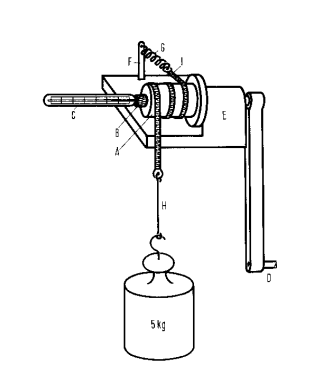
\includegraphics[width=0.2\textwidth]{bilder/Schuerholz.png}
            \caption{Schürholzapparatur}ö
        \end{figure}

		Die spezifische Wärmeänderung eines Stoffes charakterisiert die quantitativen Veränderungen der inneren Energie pro Masseneinheit, die auftreten, wenn sich die Temperatur des Stoffes entsprechend ändert. Die Spezifische Wärmekapazität misst also die Fähigkeit eines Materials, Wärmeenergie zu absorbieren oder abzugeben und dabei die Temperatur zu verändern. Diese versuchen wir im folgenden mit der Abbildung \ref{fig:abb1} zu bestimmen. Dazu wird das Kalorimeter mit Wasser befüllt und dann durch Reibung des Fadens Wärme erzeugt die in das Kalorimeter übergeht. Aus der Differenz der Wärme des Wasser im Kalorimeter lässt sich nun die Wärmeenergie bestimmen welche der Reibungsenergie entsprechen sollte.
		Dafür nutzen wir folgende Formeln:
		
		Reibungsenergie:

		$$W_{r} = F_{r} \cdot 2\pi \cdot r \cdot n$$
		
		Wärmeenergie:

		$$Q_{r} =  (\Gamma_{K} + m_{\omega}c_{\omega}) \cdot \Delta T$$
		
		Setzt man diese nun gleich lässt sich die spezifische Wärmekapazität von dem Wasser berechnen:

		$$G \cdot 2\pi \cdot r \cdot n = (m_{K}c_{K} + m_{\omega}c_{\omega}) \cdot \Delta T$$

		$$ \Rightarrow c_{\omega} = \frac{\frac{W_{r}}{\Delta T} - m_{K}c_{K}}{m_{\omega}}$$		
		
		Dies werden wir nun im folgenden Versuch durchführen.
		
	    \subsection{Versuchsdurchführung}
		
       	Die Kurbel wird je 50 mal gedrecht und nach jeden 50 mal Drehen wird die Temperatur am Thermometer abgelesen. Daraus können wir dann die Wärmeenergie sowie die Reibungsenergie berechnen. Da wir von einem geschlossen System ausgehen kann man diese wie oben gleich setzen und nach $c_{\omega}$ umstellen.
  
    \subsection{Ergebnisse}

        \begin{table}[H]
            \centering
            \begin{tabular}{|l|l|l|}
                \hline
                Anzahl der Umdrehungen $n$ & Temperatur in °C & $\Delta$ Temperatur in °C\\
                \hline
                $0$ & $22,2\ \mathrm{C}$ & $0\ \mathrm{C}$\\
                \hline
                $50$ & $23,3\ \mathrm{°C}$ & $1,1\ \mathrm{°C}$\\
                \hline
                $100$ & $24\ \mathrm{°C}$ & $0,7\ \mathrm{°C}$\\
                \hline
                $150$ & $25\ \mathrm{°C}$ & $1\ \mathrm{°C}$\\
                \hline
                $200$ & $26\ \mathrm{°C}$ & $1\ \mathrm{°C}$\\
                \hline
                $250$ & $27\ \mathrm{°C}$ & $1\ \mathrm{°C}$\\
                \hline
            \end{tabular}
        \end{table}
		$W_{r}$ lässt sich direkt aus dem Durchmesser des Kalorimeter berechnen und beträgt $339.0 J$.
        Der ermittelte Wert für die spezifische Wärmeänderung $c_{ermittelt\omega} = 3999.74 \frac{J}{kgK}$ weicht leicht vom Literaturwert für die spezifische Wärmekapazität von Wasser $c_{Lit\omega} = 4190 \frac{J}{kgK}$ ab. Diese geringfügige Diskrepanz könnte auf einzelne Messungenauigkeiten zurückgeführt werden, die sich auf das Endergebnis auswirken. Die Berechnung erfolgte durch das einzelne Berechen für $c_{\omega}$ für jedes $\Delta T$ und dann das mitteln über diese 5 Werte.
        
        Darüber hinaus ist anzumerken, dass eine hundertprozentige Energieerhaltung bei der Umwandlung von Reibungsenergie in Wärmeenergie in der Praxis nicht realisierbar ist, u.a weil das System auch Wärme an die Luft abgibt was nicht berücksichtig wird. Das kann zu weiteren Abweichungen zwischen dem gemessenen und dem theoretisch erwarteten Wert führen. Die Verfälschung des genauen Ergebnisses ist daher teilweise auf die inhärente Unvollkommenheit praktischer Energieumwandlungsprozesse zurückzuführen.  Weitre Fehlerquellen sind das anstoßen vom Thermometer am Boden(was dazu führt das die Temperatur vom Kalorimeter, welche stark von der Außentemperatur beeinflusst wird, und nicht vom Wasser gemessen wird), zu frühes ablesen vom Thermometer und Verunreinigungen vom Wasser.


\section{Versuch 2 - Vgl. verschiedener Temperaturmessmethoden}
    \subsection{Theorie Thermoelement/Widerstandsthermometer und Strahlungsthermometer}
    \subsubsection*{Thermoelement:}
    	\begin{figure}[ht]
    	\label{fig:abb2}
    	\begin{center}
    		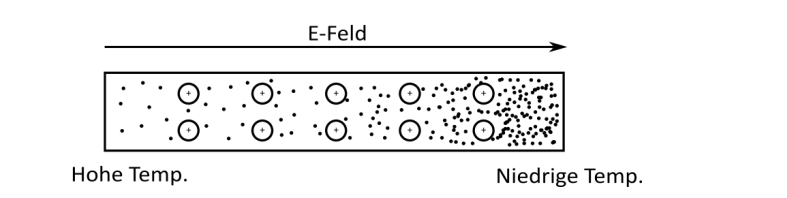
\includegraphics[width=0.5\textwidth]{bilder/Seebeck-Effekt.png}
    		\caption{Der Seebeck-Effekt vereinfacht dargestellt.}
    	\end{center}
    \end{figure}
    Durch die Anwendung eines Thermoelements ist es möglich, die Temperatur eines Stoffes zu bestimmen. Bei einem elektrischen Leiter, dessen zwei Enden unterschiedlichen Temperaturen ausgesetzt sind, entsteht aufgrund des Seebeck-Effekts eine elektrische Spannung. Dieser Effekt basiert darauf, dass Elektronen am wärmeren Ende eine höhere kinetische Energie aufweisen, wie in Abbildung \ref{fig:abb2} illustriert. Im Gegensatz dazu besitzen Elektronen am kälteren Ende eine geringere Bewegungsenergie, was zu einer höheren Elektronendichte führt. Der resultierende Unterschied in der Elektronendichte führt zu einer messbaren elektrischen Spannung.
    
   Die Höhe der gemessenen Spannung korreliert direkt mit der Größe des Temperaturunterschieds zwischen den beiden Enden des Leiters. Ein größerer Temperaturunterschied führt also zu einer höheren Spannung, die durch das Thermoelement erfasst werden kann.
   \subsubsection*{Widerstandsthermometer:}
   Das Widerstandsthermometer besteht lediglich aus einem Widerstand welcher an einem Multimeter angeschlossen ist. Taucht man diesen in die zu messende Flüssigkeit und der angezeigte Widerstand liegt zwischen 2 Werten in der Tabelle, welche in der Anleitung angehängt ist, so lässt sich durch Interpolation ein genauerer Temperaturwert bestimmen. Sei R der Widerstand und und T die Temperatur so lässt sich mit folgender Formel die gemessene Temperatur berechnen.
   $$T = T_{1} + \frac{R - R_{1}}{R_{2} - R_{1}} \cdot \Delta T$$
   \subsubsection*{Strahlungsthermometer}
   Ein Strahlungsthermometer misst die Temperatur eines Objekts, indem es die von ihm emittierte Infrarotstrahlung erfasst. Die gemessene Temperatur steht in direktem Zusammenhang mit der Temperatur des Objekts, sowie dem Abstand des Objekts zum Thermometer.  Der Abstand sollte also $\leq$ 10cm zum Objekt liegen um störende Strahlen vom Rand oder der Umgebung zu vermeiden. 
    \subsection{Versuchsaufbau und -durchführung}
	Ein Gefäß wird mit Wasser gefüllt und mit jeden der 3 Thermometer wird schnell hintereinander die Temperatur gemessen.
    \subsection{Ergebnisse}
      
	      \begin{table}[H]
		\centering
		\begin{tabular}{|l|l|}
			\hline
			Thermometerart & Gemessene T in °C\\
			\hline
			Thermoelement& 19.8 \\
			\hline
			Strahlungsthermometer & 19.6 \\
			\hline
			Widerstandsthermometer& 19.5 \\
			\hline
		\end{tabular}
	\end{table}
	Die Unterschiede zwischen den Messwerten können folgende Ursachen haben. Das Strahlenthermometer misst die Oberflächentemperatur des Wassers während die anderen 2 in der Mitte vom Wasser messen. Ein Messfehler kann die Interpolation der Widerstände sein und damit ein Unterschied zu der tatsächlichen Temperatur entstehen.
\section{Versuch 3 - Bestimmung der spezifischen Wärme von Wasser auf elektrischem Wege}
    \subsection{Theorie}
    
        	\begin{figure}[ht]
    	\label{fig:abb3}
    	\begin{center}
    		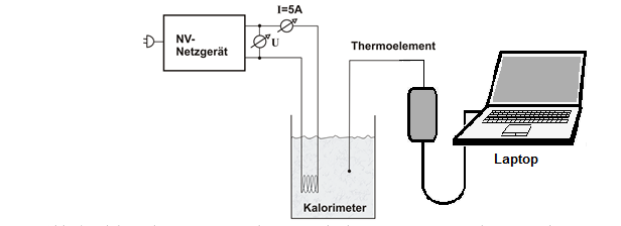
\includegraphics[width=0.6\textwidth]{bilder/Elektrisch.png}
    		\caption{Auffbau Versuch 3.}
    	\end{center}
    \end{figure}
    Die spezifische Wärmekapazität des Wassers kann auch bestimmt werden, indem man mit Hilfe der
    Joulschen Wärme, die in einem stromdurchflossenen Leiter entsteht, eine definierte Wassermenge
    erwärmt und deren Temperaturerhöhung misst, siehe Abbildung \ref{fig:abb3}. Hierzu wird eine Heizspirale ins Kalorimeter
    eingebracht, die mit einem Niedervolt-Netzgerät betrieben wird. Während des Aufheizvorgangs (5
    Minuten) werden Strom (ca. 5 A) und Spannung (ca. 10V) mit einem Amperemeter bzw. einem
    Voltmeter gemessen (wird direkt vom Gerät angezeigt). 
   Da wir von einem abgeschlossenen System ausgehen, können die zugeführte und aufgenommene
   Energie gleichgesetzt werden. Stellt man dann noch die entstandene Gleichung nach dem
   gewünschten Wert um so kann die spezifische Wärmekapazität von Wasser bestimmt werden.
   
   \noindent Hierzu benötigen die aufgenommen Wärmemenge:
   $$\Delta Q = (C_{K} + m_{Wasser}c{Wasser} ) \cdot \Delta T$$
   und die aufgewendete elektrische Arbeit:
   $$\Delta W =  U \cdot I \cdot \Delta t$$
   
   Nun lässt es sich Gleichsetzen und nach $c_{Wasser}$ umstellen:
   $$c_{Wasser} = \frac{UI\Delta t - C_{K}\Delta T}{m_{Wasser} \Delta T}$$
   
    \subsection{Ergebnisse}
	


        \begin{table}[H]
            \centering
            \begin{tabular}{|l|l|l|l|l|l|l|}
                \hline
                $G_{B}$in Kg & $G_{W}$ in Kg & Strom in A & Spannung in Volt  & $T_{1}$ in °C & $T_{2}$ in °C & $\Delta T$ in °C \\
                \hline
                 0.0995& 0.512 & 4.69 & 10.0 & 19.0 & 25.6 & 6.6 \\
                \hline
    
            \end{tabular}
        \end{table}
        Nun können wir mit der oben genannten Formel die spezifische Wärmekapazität berechnen die da wäre 3990.5 $\frac{J}{KgK}$. Die DIfferenz zum Literaturwert ist recht hoch aber lässt sich durch Fehler in der Messung erklären. 
Wir haben Folgende Fehlerquellen:
\begin{table}[H]
	\centering
	\begin{tabular}{|l|l|}
		\hline
		Fehlerquelle & Angenommener Fehler\\
		\hline
		Strom& - \\
		\hline
		Spannung& -\\
		\hline
		Masse Wasser& 0.0001kg \\
		\hline
		Zeit & 1s\\
		\hline
		Temperatur & 0.2°C\\
	 \hline
	\end{tabular}
\end{table}
Daraus können wir folgenden Gesamtfehler berechnen:

$$\Delta c_{Wasser}  = \left| \frac{U I \Delta t}{m_{Wasser} \Delta T^2} \right| \cdot \delta T + \left| \frac{I U}{m_{Wasser} \Delta T} \right| \delta t +  \left| \frac{\frac{-U I \Delta t}{\Delta T} - m_{k}c_{k}}{m^2_{Wasser}} \cdot \right| \Delta m_{Wasser}  $$

Der Größtfehler beträgt $140.87 \frac{J}{KgK}$. Draus folgt ein Ergebnis von $ 3990.5 \frac{J}{KgK} \pm 140.87 \frac{J}{KgK}$ was recht nah am Literaturwert liegt.  Zusätzlich werden die Wärmeverluste bei diesem Versuch nicht berücksichtigt, was ebenfalls zu einer Abweichung führt. 
\section{Versuch 4 - Spezifische Wärmekapazität fester Körper}
	    \subsection{Theorie}
	Die spezifische Wärmekapazität fester Körper wird mittels der Mischungsmethode bestimmt, indem ein Probekörper der Masse $m_{1}$ auf die Temperatur von siedendem Wasser erhitzt wird und anschließend in ein Kalorimeter mit Wasser der Masse $m_{2}$ und Anfangstemperatur $T_{1}$ gebracht wird. Die Entwicklung der Mischtemperatur $T_{misch}$ aufgezeichnet wird aufgezeichnet und draus die Wärmekapazität des Körpers berechnet.
	
	Dazu benötigt man die vom Körper abgegeben Wärmeenergie:
	$$\Delta Q_{1} = m_{1}c_{1} \cdot (T_{1} - T_{misch})$$
	wobei $c_{1}$ die spezifische Wärmekapazität ist die berechnet werden soll. Die im Kalorimeter aufgenommen Wärmemenge lässt sich mit:
	$$\Delta Q_{2} = (C_{K} + m_{2}c_{Wasser}) \cdot (T_{misch} - T_{2})$$
	berechnen.
	
	Da wir von einem abgeschlossenen System ausgehen lässt sich $c_{1}$ durch Gleichsetzen von $Q_{1} = Q_{2}$ und umstellen tatsächlich berechnen:
	$$c_{1} = \frac{(C_{K} +m_{2}c_{Wasser}) \cdot (T_{misch} - T_{2})}{m_{1} \cdot (T_{1} - T_{misch})}$$
	
	Der Aufbau sieht in etwa so aus:
	       	\begin{figure}[ht]
		\label{fig:abb4}
		\begin{center}
			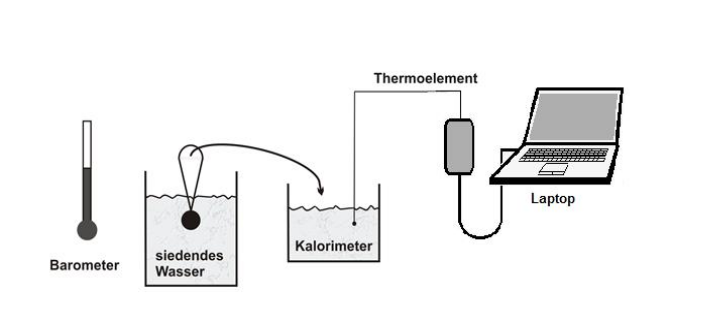
\includegraphics[width=0.6\textwidth]{bilder/Fest.png}
			\caption{Auffbau Versuch 4.}
		\end{center}
	\end{figure}
    \subsection{Versuchsdurchführung}
  Zuerst wird derLuftdruck mit einem Barometer bestimmt um den Siedepunkt des Wasser zu bestimmen. Dann wird der Köper gewogen und im Wasser auf Temperatur gebracht.  Nun lässt sich mit durch den Temperaturunterschied vom Wasser die spezifische Wärmekapazität mihilfe von oben genannter Formel berechnen. 
    \subsection{Ergebnisse}
	Die Masse der Körper beträgt:
	\begin{table}[H]
		\centering
		\begin{tabular}{|l|l|}
			\hline
		 	Probekörperart & Gewicht in Kg\\
			\hline
			Eisen & 0.107\\
			\hline
			Messing& 0.116\\
			\hline
			Aluminium& 0.108\\
			\hline
			Kalorimeter& 0.1006\\
			\hline
			Wasser& 0.5551\\
			\hline
		\end{tabular}
	\end{table}
	Da wir einen Luftdruck von 960mBar haben wir eine Siedtemperatur 98.9°C.
        \begin{table}[H]
            \centering
            \begin{tabular}{|l|l|l|}
                \hline
                Metallart  & Wasser Temp $T_{1}$ & Wassertemp $ \Delta T$\\
                \hline
                Aluminium& 19.7 & 22.6\\
                \hline
                Messing &  22.6  & 23.9 \\
                \hline
                Eisen& 23.8 & 25.3\\
                \hline
            \end{tabular}
        \end{table}
        Nun können wir folgende Werte durch einsetzen in unsere Formel oben berechnen:
        \begin{table}[H]
        	\centering
        	\begin{tabular}{|l|l|l|l|}
        		\hline
        		Metallart & Literaturwert $(\frac{J}{KgK})$ & Berechnet $(\frac{J}{KgK})$ & Abweichung $(\frac{J}{KgK})$ \\
        		\hline
        		Eisen& 450 & 445.3 & 4.7\\
        		\hline
        		Messing & 381& 349.3 & 31.7 \\
        		\hline
        		Aluminium& 896 & 794.4 & 101.6 \\
        		\hline
        	\end{tabular}
        \end{table}
Die Abweichungen ergeben sich aus den Messfehlern beim ablesen, durch zu langsames rübertragen vom  kochenden Wasser in das Kalorimeter oder zu frühes entfernen vom Körper aus diesem. 


\section{Versuch 5 - Latente Wärme - die spezifische Schmelzwärme von Wassser}
    \subsection{Theorie}
    Kommt es bei der Abgabe oder Aufnahme von Wärmeenergie zu einer Strukturumwandlung (zb schmelzen von Eis), so bleibt dabei die Temperatur konstant. Diese Wärmeenergie wird auch latente Wärme bezeichnet. Die spezifische Schmelzwärme $q_s$ eines Stoffs ist der Quotient aus der zu Schmelzen zugeführten Wärmeenergie und der Masse des Stoffs. 
    $$q_s = \frac{\Delta Q_s}{m}$$
    
    Wärme die das Kalorimeter abgibt:
    
    $$\Delta Q_{abgegeben} = (m_{Wasser}c_{Wasser} + C_{Kalorimeter}) (T_1 - T_{misch})$$
    
    Und die vom Eis/Schmelzwasser aufgenommene Wärme beträgt:
    
    $$\Delta Q_{aufgenommen} = m_{Eis}q_s + m_{Eis} c_{Wasser}(T_{misch} - T_{Eis})$$
    
    In diesem Versuch nehmen wir $T_{Eis} = 0 \text{°C}$ an. Nun lässt sich $\Delta Q_{aufgenommen}$ und $\Delta Q_{abgegeben} $ gleichsetzen und nach $q_s$ umstellen. Daraus folgt dann: 
    
    $$\Delta q_s = \frac{(m_{Wasser}c_{Wasser} + C_{Kalorimeter}) (T_1 - T_{misch}) - m_{Eis} c_{Wasser}(T_{misch} - T_{Eis})}{m_{Eis}}$$
    \subsection{Versuchsaufbau und -durchführung}
     In diesem Versuch soll die Schmelzwärme von Wasser bestimmt werden. Dazu wird Eis in warmen Wasser geschmolzen. Zu Beginn wird die die MAsse vom Kalorimeter und dem Eis gewogen. Danach wird das Eis hinzugefügt und die Gesamtmasse erneut gewogen.
     Dann lässt sich mit den oben genannten Formeln die Schmelzwärme bestimmen.

    
    \subsection{Ergebnisse}

        Die Messwerte sind in der folgenden Tabelle aufgelistet:

        \begin{table}[H]
            \centering
            \begin{tabular}{|l|l|}
                \hline
                 & Messwerte\\
                \hline
                Gewicht Wasser warm $m_{Wasser}$ & 0.5144 kg\\
                \hline
                Gewicht Eis $m_{Eis}$ &0.2178 kg\\
                \hline
                Temperatur $T_1$ & 39.0 °C \\
            \hline
            Temperatur $T_{misch}$ & 19.2 °C \\
            \hline
            \end{tabular}
        \end{table}
        Mit oben genannter Formel kommen wir auf eine Schmelzwärme von: 
        283326 $J/Kg$
        
		Abweichungen sind darauf
		zurückzuführen, dass hier wieder eine Idealisierung vorgenommen wurde.
		Das System tauscht zusätzlich Wärme mit der Umgebung aus. Diese wird
		nicht berücksichtigt und verfälscht somit das Ergebnis. Zu begin ist außerdem beim Eis eine bestimmte Menge Schmelzwasser vorhanden
		was hier aber noch zur Masse des Eises gerechnet wird.
